\chapter{Derivative-Free Optimization}
\label{chap:derivative-free}
\textit{(Brent, 1973)}

\section{Introduction}

Often, derivatives are unavailable or difficult to compute.
Examples:
\begin{itemize}
    \item The result of an experimental measurement.
    \item The result of a stochastic simulation.
    \item $f$ is known but computing the derivatives is too expensive.
\end{itemize}

\section{Some Possible Solutions}

\begin{itemize}
    \item \textbf{Automatic differentiation}: if a binary code computes $f$, we can apply automatic differentiation.
    
    \textit{Principle.} If $f(x) = g(h(m(x)))$, we denote $w = m(x)$, $y = h(w)$, $z = g(y)$.
    We use the \textit{chain rule}:
    \[
        f'(x) = \frac{\partial g}{\partial y} \bigg|_y \times \frac{\partial h}{\partial w} \bigg|_w \times \frac{\partial m}{\partial x} \bigg|_x.
    \]

    \item \textbf{Finite differences}: use finite differences to approximate $\nabla f$ (and perhaps $\nabla^2 f$), then apply the algorithms from the previous chapters.
    \textbf{But} this may be impossible due to approximations or \textit{noise}.
\end{itemize}

\section{The Problem of Noise}

In many applications, the objective function looks like:
\begin{equation}
    f(x) = h(x) + \phi(x),
\end{equation}
where $h$ is a smooth (differentiable) function, and $\phi$ represents the noise (possibly independent of $x$).

The finite difference approximation of the gradient $\nabla f(x)$ for $\epsilon > 0$ is given by:
\[
    \nabla_\epsilon f(x) = \left( \frac{f(x+\epsilon e_i) - f(x-\epsilon e_i)}{2\epsilon} \right)_{i=1,\dots,n},
\]
where $e_i = (0, \dots, 1, \dots, 0)^\top$ is the $i$-th vector of the canonical basis.

\subsection{Noise Level and Approximation Error}

Let us define the local noise level $\eta(x, \epsilon)$ by:
\begin{equation}
    \eta(x, \epsilon) = \sup_{\|z-x\|_\infty < \epsilon} |\phi(z)|.
\end{equation}

\begin{figure}[H]
\centering
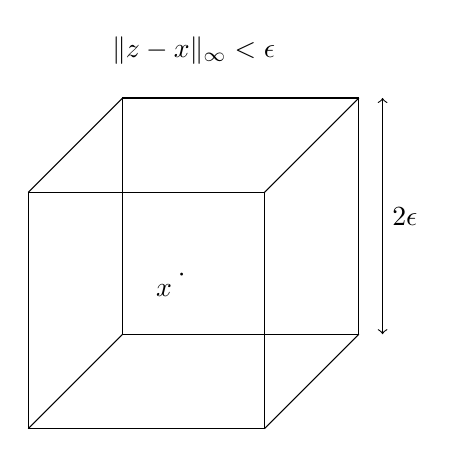
\begin{tikzpicture}[scale=1.5]
    % Simple 3D cube
    \draw (0,0) rectangle (2,2); % Front face
    % x positioned more towards center of the 3D cube (accounting for perspective)
    \draw (1.3,1.3) node {$\cdot$} node[below left] {$x$};
    
    \draw (0,0) -- (0.8,0.8);
    \draw (2,0) -- (2.8,0.8);
    \draw (0,2) -- (0.8,2.8);
    \draw (2,2) -- (2.8,2.8);
    
    \draw (0.8,0.8) -- (2.8,0.8) -- (2.8,2.8) -- (0.8,2.8) -- cycle; % Back face
    
    % Dimensions
    \draw[<->] (3.0, 0.8) -- (3.0, 2.8) node[midway, right] {$2\epsilon$};
    
    \node at (1.4, 3.2) {$\|z - x\|_\infty < \epsilon$};
\end{tikzpicture}
\caption{Neighborhood considered for the noise level.}
\label{fig:noise-cube}
\end{figure}

\begin{figureexplanation}
Figure~\ref{fig:noise-cube} represents the cubic neighborhood $\|z - x\|_\infty < \epsilon$ around the point $x$. The local noise level $\eta(x, \epsilon)$ corresponds to the largest amplitude of the noise $\phi(z)$ encountered inside this cube of side $2\epsilon$.
\end{figureexplanation}

It can be shown that if $\nabla^2 h$ is $L$-Lipschitz continuous in the neighborhood $\{z \mid \|z-x\|_\infty < \epsilon\}$, then:
\begin{equation}
    \|\nabla_\epsilon f(x) - \nabla h(x)\|_\infty \le \underbrace{L \epsilon^2}_{\text{finite differences}} + \underbrace{\frac{\eta(x, \epsilon)}{\epsilon}}_{\text{noise}}.
\end{equation}

Thus, one cannot expect a good approximation of $\nabla h(x)$ if the noise is significant, because reducing $\epsilon$ increases the amplification of the noise ($\eta/\epsilon$).

\begin{figure}[H]
\centering
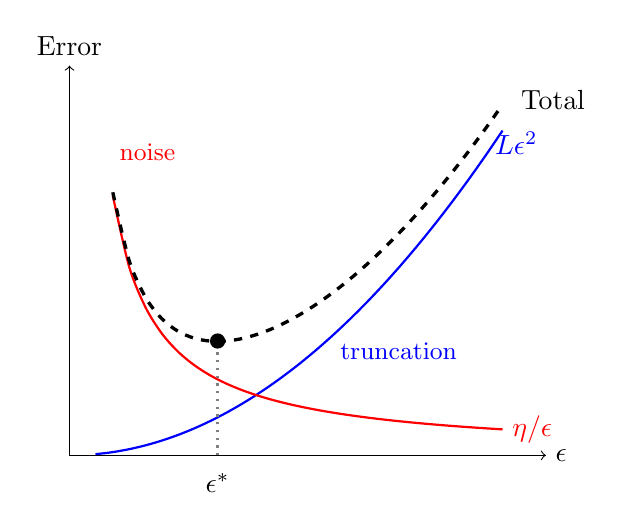
\begin{tikzpicture}[scale=1.1]
    % Axes
    \draw[->] (0,0) -- (5.5,0) node[right] {$\epsilon$};
    \draw[->] (0,0) -- (0,4.5) node[above] {Error};
    
    % Truncation error: L*epsilon^2 (quadratic, small near 0)
    \draw[domain=0.3:5, smooth, variable=\x, blue, thick] 
        plot ({\x}, {0.15*\x*\x});
    \node[blue, right] at (4.8, 3.6) {$L\epsilon^2$};
    \node[blue] at (3.8, 1.2) {\small truncation};
    
    % Noise amplification: eta/epsilon (hyperbolic, large near 0)
    \draw[domain=0.5:5, smooth, variable=\x, red, thick] 
        plot ({\x}, {1.5/\x});
    \node[red, right] at (5, 0.3) {$\eta/\epsilon$};
    \node[red] at (0.9, 3.5) {\small noise};
    
    % Total error (sum)
    \draw[domain=0.5:5, smooth, variable=\x, black, very thick, dashed] 
        plot ({\x}, {0.15*\x*\x + 1.5/\x});
    \node[right] at (5.1, 4.1) {Total};
    
    % Optimal epsilon (minimum of total)
    % Derivative: 0.3*eps - 1.5/eps^2 = 0 => eps^3 = 5 => eps ~ 1.71
    \draw[dotted, gray, thick] (1.71, 0) -- (1.71, 1.32);
    \node[below] at (1.71, -0.1) {$\epsilon^*$};
    \fill (1.71, 1.32) circle (2.5pt);
\end{tikzpicture}
\caption{Trade-off truncation error vs noise amplification. The total error (dashed) has a minimum at $\epsilon^*$.}
\label{fig:error-epsilon}
\end{figure}

\subsection{Example: Stochastic Noise}

Let $X_1, \dots, X_n$ be i.i.d. (independent and identically distributed) random variables with a mean $h(x)$ and a finite variance $\sigma^2$.

Then the Central Limit Theorem gives:
\[
    \sqrt{n} \left( \frac{1}{n} \sum_{i=1}^n X_i - h(x) \right) \xrightarrow{d} \mathcal{N}(0, \sigma^2).
\]
Roughly:
\[
    \frac{1}{n} \sum_{i=1}^n X_i - h(x) \approx \frac{\sigma}{\sqrt{n}} G,
\]
where $G \sim \mathcal{N}(0, 1)$.
This shows that the error decreases only as $1/\sqrt{n}$, which may require a very large number of samples to reduce the noise to an acceptable level for finite differences.

So that:
\[
    \underbrace{\frac{1}{n} \sum_{i=1}^n X_i}_{\text{observed}}
    \simeq
    \underbrace{h(x)}_{\text{useful part}}
    +
    \underbrace{\frac{\sigma}{\sqrt{n}} G}_{\text{noise } \phi}.
\]
In this situation, $\phi$ is independent of $x$, and $\phi$ is even unbounded (since the normal distribution is unbounded).

\begin{quote}
    \textbf{Caution:} From now on, we assume that $f$ has continuous derivatives, even though these will not be used in the algorithms.
\end{quote}

We propose a non-exhaustive selection of methods.

\section{Model-based methods}

\subsection{General Idea}
The idea is to build a model $m_k$ (often quadratic) that interpolates the function $f$ on a set of well-chosen points.

Suppose that at step $k$, we have an interpolation set of points $\mathcal{Y} = \{y_1, \dots, y_q\}$ with $y_i \in \mathbb{R}^n$ for $i=1, \dots, q$, and that the current iterate $x_k$ is one of them. Moreover, no point in $\mathcal{Y}$ has a function value lower than $f(x_k)$.

\subsection{Building the model}

Our model will be of the form:
\begin{equation}
    m_k(x_k + p) = c + g^\top p + \frac{1}{2} p^\top G p,
\end{equation}
where $c \in \mathbb{R}$, $g \in \mathbb{R}^n$, and $G \in \mathbb{R}^{n \times n}$ is symmetric.

We determine $c$, $g$ and $G$ by imposing the interpolation conditions:
\begin{equation}
    m_k(y_i) = f(y_i), \quad i=1, \dots, q.
\end{equation}

There are $1 + n + \frac{n(n+1)}{2} = \frac{(n+1)(n+2)}{2}$ coefficients to adjust.
If we choose $q = \frac{(n+1)(n+2)}{2}$, the system admits a unique solution (provided the points are well positioned).

Then, we compute the step $p$ by solving the trust-region subproblem:
\begin{equation}
    \min_p m_k(x_k + p) \quad \text{subject to } \|p\|_2 \le \Delta,
\end{equation}
for some trust-region radius $\Delta$.

\subsection{Update}
\begin{itemize}
    \item If the decrease is "significant", we will increase $\Delta$ for the next iteration.
    \item Otherwise, we update the set $\mathcal{Y}$ or reduce the trust-region radius $\Delta$, and reject the step.
\end{itemize}

\subsection{Initialization and Geometry}
For the complete algorithm (Algorithm 13), initialization is often done by taking the $n+1$ vertices and the $\frac{n(n+1)}{2}$ edge midpoints of a simplex in $\mathbb{R}^n$.

\begin{definition}[Simplex]
    A simplex in $\mathbb{R}^n$ is a set of $n+1$ vectors $y_1, \dots, y_{n+1}$ in $\mathbb{R}^n$.
    
    The simplex $\{y_1, \dots, y_{n+1}\}$ is called \textbf{non-degenerate} if the matrix
    \[
        \begin{bmatrix}
            y_2 - y_1 & y_3 - y_1 & \cdots & y_{n+1} - y_1
        \end{bmatrix}
    \]
    is non-singular (i.e., the directions are independent).
\end{definition}

\begin{figure}[H]
\centering
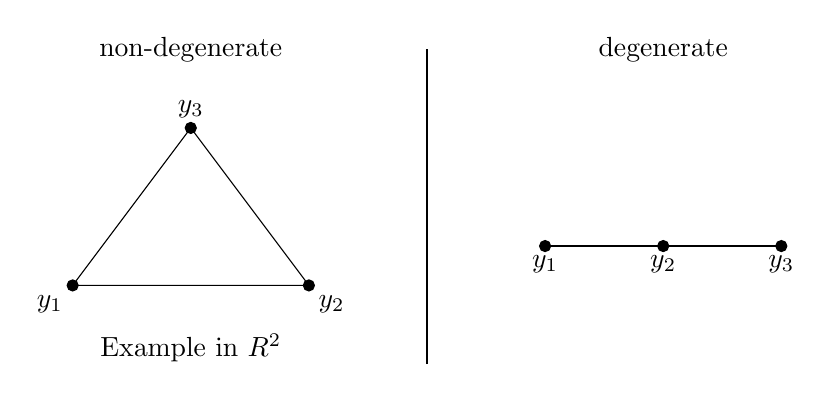
\begin{tikzpicture}[scale=1.0]
    % Non-degenerate simplex (Triangle) in R^2
    \begin{scope}[shift={(0,0)}]
        \node at (1.5, 3.0) {non-degenerate};
        \coordinate (A) at (0,0);
        \coordinate (B) at (3,0);
        \coordinate (C) at (1.5, 2);
        
        \draw (A) -- (B) -- (C) -- cycle;
        
        \filldraw (A) circle (2pt) node[below left] {$y_1$};
        \filldraw (B) circle (2pt) node[below right] {$y_2$};
        \filldraw (C) circle (2pt) node[above] {$y_3$};
        
        \node at (1.5, -0.8) {Example in $\mathbb{R}^2$};
    \end{scope}
    
    % Vertical separator line
    \draw (4.5, -1) -- (4.5, 3);
    
    % Degenerate simplex (Aligned points)
    \begin{scope}[shift={(6,0)}]
        \node at (1.5, 3.0) {degenerate};
        \coordinate (D) at (0, 0.5);
        \coordinate (E) at (1.5, 0.5);
        \coordinate (F) at (3, 0.5);
        
        \draw (D) -- (F); % Line connecting them
        
        \filldraw (D) circle (2pt) node[below] {$y_1$};
        \filldraw (E) circle (2pt) node[below] {$y_2$};
        \filldraw (F) circle (2pt) node[below] {$y_3$};
    \end{scope}
\end{tikzpicture}
\caption{Illustration of a non-degenerate vs degenerate simplex in $\mathbb{R}^2$.}
\label{fig:simplex-degenerate}
\end{figure}

\begin{figureexplanation}
Figure~\ref{fig:simplex-degenerate} illustrates the concept of degeneracy. On the left, the vectors $y_2-y_1$ and $y_3-y_1$ are linearly independent, forming a true triangle (non-zero volume). On the right, the points are collinear: the vectors are collinear, the associated matrix is singular, and the simplex is degenerate (zero volume).
\end{figureexplanation}

\begin{algorithm}[H]
\caption{Model-Based Derivative-Free Method}
\label{alg:model-based-dfo}
Choose an interpolation set $Y = \{y^1, \ldots, y^q\}$ such that the linear system defined by $m_k(y^\ell) = f(y^\ell), \ell = 1, \ldots, q$ is nonsingular, and select $x_0$ as a point in this set such that $f(x_0) \le f(y^i)$ for all $y^i \in Y$. Choose an initial trust region radius $\Delta_0$, a constant $\eta \in (0,1)$, and set $k \leftarrow 0$\;
\Repeat{a convergence test is satisfied}{
    Form the quadratic model $m_k(x_k+p)$ that satisfies the interpolation conditions $m_k(y^\ell) = f(y^\ell), \ell = 1, \ldots, q$\;
    Compute a step $p$ by approximately solving $\min_p m_k(x_k + p)$, subject to $\|p\|_2 \le \Delta_k$\;
    Define the trial point $x_k^+ = x_k + p$\;
    Compute the ratio $\rho = \dfrac{f(x_k) - f(x_k^+)}{m_k(x_k) - m_k(x_k^+)}$\;
    \If{$\rho \ge \eta$}{
        Replace an element of $Y$ by $x_k^+$\;
        Choose $\Delta_{k+1} \ge \Delta_k$\;
        Set $x_{k+1} \leftarrow x_k^+$\;
        Set $k \leftarrow k+1$ and go to the next iteration\;
    }
    \ElseIf{the set $Y$ need not be improved}{
        Choose $\Delta_{k+1} < \Delta_k$\;
        Set $x_{k+1} \leftarrow x_k$\;
        Set $k \leftarrow k+1$ and go to the next iteration\;
    }
    Invoke a geometry-improving procedure to update $Y$: at least one of the points in $Y$ is replaced by some other point, with the goal of improving the conditioning of $m_k(y^\ell) = f(y^\ell), \ell = 1, \ldots, q$\;
    Set $\Delta_{k+1} \leftarrow \Delta_k$\;
    Set $x_k^+ \leftarrow \hat{x}$ and recompute $\rho$ by $\rho = \dfrac{f(x_k) - f(x_k^+)}{m_k(x_k) - m_k(x_k^+)}$\;
    \If{$\rho \ge \eta$}{
        Set $x_{k+1} \leftarrow x_k^+$\;
    }
    \Else{
        Set $x_{k+1} \leftarrow x_k$\;
    }
    $k \leftarrow k + 1$\;
}
\end{algorithm}

\section{Coordinate or pattern-search methods}

Starting from the current iterate, we look at certain points along specified directions, and we decide the step.

\subsection{Coordinate search}
Also called \textit{coordinate descent}.

\paragraph{Idea.}
We cycle through the $n$ coordinate directions $e_1, \dots, e_n$.
We minimize $f$ along $e_i$, then we start again...

\paragraph{Warning.}
This method may never approach a point where the gradient vanishes (\textit{gradient-vanishing point})!
It can stagnate at the corners of sharp level contours if the directions are not adapted to the local geometry of the function.

When convergence does occur, it may be slower than \textit{steepest descent}.

\begin{figure}[H]
\centering
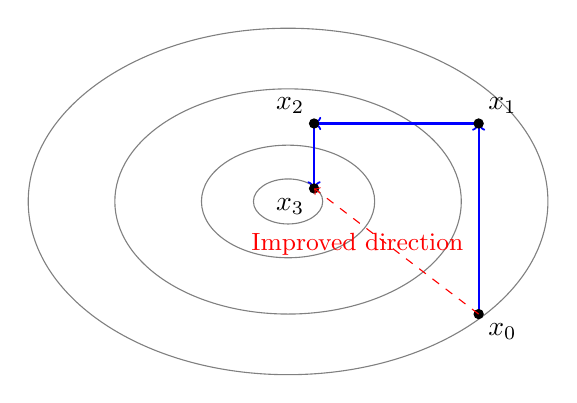
\begin{tikzpicture}[scale=1.1]
    % Contours (ellipses) - centered at origin
    \draw[gray] (0,0) ellipse (3cm and 2cm);
    \draw[gray] (0,0) ellipse (2cm and 1.3cm);
    \draw[gray] (0,0) ellipse (1cm and 0.65cm);
    \draw[gray] (0,0) ellipse (0.4cm and 0.26cm);

    % Starting point x0 on the outer ellipse
    % Ellipse: (x/3)^2 + (y/2)^2 = 1
    % At x=2.2: (2.2/3)^2 + (y/2)^2 = 1 => y = 2*sqrt(1-0.537) = 1.36
    % Let's place x0 at (2.2, -1.3) approximately on outer ellipse
    
    \coordinate (x0) at (2.2, -1.3);
    % Move vertically (along y) - coordinate search along e2
    \coordinate (x1) at (2.2, 0.9);
    % Move horizontally (along x) - coordinate search along e1
    \coordinate (x2) at (0.3, 0.9);
    % Move vertically again
    \coordinate (x3) at (0.3, 0.15);

    % Zigzag path with arrows
    \draw[->, thick, blue] (x0) -- (x1);
    \draw[->, thick, blue] (x1) -- (x2);
    \draw[->, thick, blue] (x2) -- (x3);

    % Point labels
    \node[below right] at (x0) {$x_0$};
    \node[above right] at (x1) {$x_1$};
    \node[above left] at (x2) {$x_2$};
    \node[below left] at (x3) {$x_3$};
    
    % Points markers
    \filldraw (x0) circle (1.5pt);
    \filldraw (x1) circle (1.5pt);
    \filldraw (x2) circle (1.5pt);
    \filldraw (x3) circle (1.5pt);

    % Improvement direction (direct path)
    \draw[dashed, red, ->] (x0) -- (x3);
    \node[red] at (0.8, -0.5) {\small Improved direction};
\end{tikzpicture}
\caption{Illustration of coordinate search (zigzag) and its potential slowness.}
\label{fig:coordinate-zigzag}
\end{figure}

\begin{figureexplanation}
Figure~\ref{fig:coordinate-zigzag} shows that the method progresses in steps (zigzag). The coordinate directions do not necessarily point perfectly toward the minimum, forcing many small steps.
\end{figureexplanation}

\paragraph{Possible Improvement.}
Perform $n$ iterations and then run a line search along the direction $(x_k - x_{k-n})$.
\subsection{Pattern-search methods}

This class of methods generalizes the previous approach.

\paragraph{Idea.}
Choose a set of search directions $D_k$, and at each iteration, evaluate $f$ at a given step length $\gamma_k$ along these directions.
If a "more interesting" point is found, it becomes the new iterate.

\subsubsection{Algorithm 14 (General Scheme)}
It can be shown that there exist stationary accumulation points.
At step $k$, let $x_k$ be the current iterate, $D_k$ the current set of directions, and $\gamma_k$ the step length.

\begin{itemize}
    \item \textbf{Success:} If one of the directions in $D_k$ produces a significant decrease, we move to this new point and increase the step $\gamma_k$.
    \item \textbf{Failure:} Otherwise, we keep $x_k$ and decrease $\gamma_k$.
    \item Under certain conditions, the set $D_k$ can be modified.
\end{itemize}

\subsubsection{Conditions on $D_k$}
To ensure convergence, the set $D_k$ must sufficiently cover the space.
There must be at least one descent direction in $D_k$, meaning a direction $d \in D_k$ such that:
\[
    \cos(\theta) = \frac{-\nabla f_k^\top d}{\|\nabla f_k\| \|d\|} > 0
\]

\paragraph{Zoutendijk's Condition (adapted).}
Let us ensure that there exists $\delta > 0$ such that $\cos(\theta) > \delta$ for at least one direction.
We define the quality measure of the set of directions $\kappa(D_k)$ by:
\begin{equation}
    \kappa(D_k) = \min_{v \in \mathbb{R}^n} \max_{p \in D_k} \frac{v^\top p}{\|v\| \|p\|}
\end{equation}
The condition is then: $\kappa(D_k) \ge \delta > 0$.

\textit{Interpretation:} This condition means that for any vector $v$, there exists a direction $p \in D_k$ that forms an angle "sufficiently far" from $\pi/2$ with $v$. More precisely, the cosine of the angle between $v$ and $p$ is bounded from below by a strictly positive constant $\delta$.

\subsubsection{Bounds on the step}
There must exist positive constants $\underline{\beta}, \bar{\beta}$ such that for all $p \in D_k$:
\[
    \underline{\beta} \le \|p\|_2 \le \bar{\beta}
\]
The step $\gamma_k$ must capture the effective diameter of the search.

Under these two conditions, for any $k$, there exists a vector $p \in D_k$ such that:
\begin{equation}
    -\nabla f_k^\top p \ge \kappa(D_k) \|\nabla f_k\| \|p\| \ge \delta \|\nabla f_k\| \underline{\beta}
\end{equation}
This guarantees a sufficient decrease as long as the gradient is not zero.

\subsubsection{Possible Sets $D_k$ satisfying these conditions}

Here are a few examples of sets $D_k$ that satisfy the stated conditions:

\paragraph{Example 1: Canonical directions and their opposites.}
\begin{equation}
    D_k = \{e_1, -e_1, e_2, -e_2, \dots, e_n, -e_n\}
\end{equation}
where $e_i$ is the $i$-th vector of the canonical basis.

\begin{figure}[H]
\centering
\begin{tikzpicture}[scale=1.2]
    % Axes for 2D case
    \draw[->, thick] (-2,0) -- (2,0) node[right] {$e_1$};
    \draw[->, thick] (0,-2) -- (0,2) node[above] {$e_2$};
    
    % Direction arrows
    \draw[->, blue, very thick] (0,0) -- (1.5,0) node[above right] {$e_1$};
    \draw[->, blue, very thick] (0,0) -- (-1.5,0) node[above left] {$-e_1$};
    \draw[->, red, very thick] (0,0) -- (0,1.5) node[above right] {$e_2$};
    \draw[->, red, very thick] (0,0) -- (0,-1.5) node[below right] {$-e_2$};
    
    \node at (0,-2.5) {Case $n = 2$};
\end{tikzpicture}
\caption{Direction set $D_k = \{e_1, -e_1, e_2, -e_2\}$ in $\mathbb{R}^2$.}
\label{fig:dk-canonical}
\end{figure}

\paragraph{Example 2: Simplex directions.}
For $n \geq 1$, we define:
\begin{align}
    n_i &= \frac{1}{2n} e - e_i, \quad i = 1, \dots, n, \\
    n_{n+1} &= \frac{1}{2n} e,
\end{align}
where $e = (1, \dots, 1)^\top \in \mathbb{R}^n$.

\begin{figure}[H]
\centering
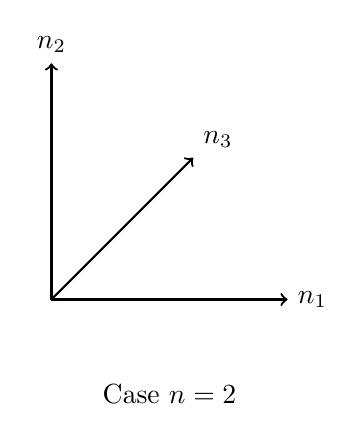
\begin{tikzpicture}[scale=1.5]
    % 3D coordinate system for illustration
    \draw[->, thick] (0,0) -- (2,0) node[right] {$n_1$};
    \draw[->, thick] (0,0) -- (0,2) node[above] {$n_2$};
    \draw[->, thick] (0,0) -- (1.2,1.2) node[above right] {$n_3$};
    
    \node at (1,-0.8) {Case $n = 2$};
\end{tikzpicture}
\caption{Simplex directions in $\mathbb{R}^2$.}
\label{fig:dk-simplex-directions}
\end{figure}

\begin{remarque}
\begin{itemize}
    \item One can always enrich the set $D_k$ with interesting heuristics.
    \item It is not necessary to examine all directions at every step.
\end{itemize}
\end{remarque}

\begin{algorithm}[H]
\caption{Pattern search method}
\label{alg:pattern-search}
Given convergence tolerance $\gamma_{\text{tol}}$, contraction parameter $\theta_{\max}$, sufficient decrease function $\rho : [0,\infty) \to \mathbf{R}$ with $\rho$ an increasing function and $\frac{\rho(t)}{t} \to 0$ as $t \downarrow 0$\;
Choose initial point $x_0$, initial step length $\gamma_0 > \gamma_{\text{tol}}$, initial direction set $\mathcal{D}_0$\;
\For{$k = 1, 2, \ldots$}{
    \If{$\gamma_k \le \gamma_{\text{tol}}$}{
        \Stop\;
    }
    \If{$f(x_k + \gamma_k p_k) < f(x_k) - \rho(\gamma_k)$ for some $p_k \in \mathcal{D}_k$}{
        Set $x_{k+1} \leftarrow x_k + \gamma_k p_k$ for some such $p_k$\;
        Set $\gamma_{k+1} \leftarrow \phi_k \gamma_k$ for some $\phi_k \ge 1$ \Comment*[r]{increase step length}
    }
    \Else{
        Set $x_{k+1} \leftarrow x_k$\;
        Set $\gamma_{k+1} \leftarrow \theta_k \gamma_k$, where $0 < \theta_k \le \theta_{\max} < 1$\;
    }
}
\end{algorithm}

\section{Nelder-Mead Simplex Method}

\subsection{General Principle}

At each step, we keep track of $n+1$ points in $\mathbb{R}^n$, which form a simplex.

At each iteration:
\begin{itemize}
    \item We remove a point from the simplex.
    \item We replace it with a point located on the line connecting the old point to the centroid of the $n$ best points.
    \item The simplex will be \textbf{expanded}, \textbf{reflected}, or \textbf{contracted}.
\end{itemize}

If there is no such point that improves the function, we \textbf{shrink} the simplex towards the best point.

\subsection{Notation and Ordering}

At a given step, suppose the vertices of the simplex are ordered by increasing function value:
\begin{equation}
    f(x_1) \leq f(x_2) \leq \cdots \leq f(x_{n+1})
\end{equation}
Thus, $x_1$ is the best point (smallest value of $f$), and $x_{n+1}$ is the worst point.

\subsection{Centroid}

The centroid of the $n$ best points (i.e., all except $x_{n+1}$) is:
\begin{equation}
    \bar{x} = \frac{1}{n} \sum_{i=1}^{n} x_i
\end{equation}

\subsection{Candidate Points}

The points on the line connecting $x_{n+1}$ and $\bar{x}$ are given by:
\begin{equation}
    \bar{x}(t) = \bar{x} + t(x_{n+1} - \bar{x}), \quad t \in \mathbb{R}
\end{equation}

\begin{figure}[H]
\centering
\begin{tikzpicture}[scale=1.3]
    % Simplex vertices
    \coordinate (x1) at (0, 0);
    \coordinate (x2) at (3, 0.3);
    \coordinate (x3) at (1.5, 2.5);
    
    % Centroid of x1 and x2
    \coordinate (xbar) at (1.5, 0.15);
    
    % Draw simplex
    \draw[thick] (x1) -- (x2) -- (x3) -- cycle;
    
    % Points
    \filldraw (x1) circle (2pt) node[below left] {$x_1$};
    \filldraw (x2) circle (2pt) node[below right] {$x_2$};
    \filldraw (x3) circle (2pt) node[above] {$x_3 = x_{n+1}$};
    \filldraw[blue] (xbar) circle (2pt) node[below] {$\bar{x}$};
    
    % Line from xbar through x3 and beyond
    % Extend the line: from t=-2 (below xbar) to t=1 (at x3)
    \draw[dashed, gray] ($(xbar)!-2!(x3)$) -- ($(xbar)!1.2!(x3)$);
    
    % Candidate points - TikZ (A)!t!(B) = A + t*(B-A)
    % which matches x̄(t) = x̄ + t*(x_{n+1} - x̄)
    \coordinate (xm2) at ($(xbar)!-2!(x3)$);     % t = -2 (expansion)
    \coordinate (xm1) at ($(xbar)!-1!(x3)$);     % t = -1 (reflection)
    \coordinate (xmhalf) at ($(xbar)!-0.5!(x3)$); % t = -1/2 (outside contraction)
    \coordinate (xphalf) at ($(xbar)!0.5!(x3)$);  % t = 1/2 (inside contraction)
    
    \filldraw[red] (xm2) circle (2pt) node[below] {$\bar{x}(-2)$};
    \filldraw[red] (xm1) circle (2pt) node[left] {$\bar{x}(-1)$};
    \filldraw[orange] (xmhalf) circle (2pt) node[left] {$\bar{x}(-\frac{1}{2})$};
    \filldraw[orange] (xphalf) circle (2pt) node[right] {$\bar{x}(\frac{1}{2})$};
    
    % Labels
    \node at (5, 1.5) {\small $t < 0$: reflection/expansion};
    \node at (5, 1) {\small $t > 0$: contraction};
\end{tikzpicture}
\caption{Candidate points on the line connecting $x_{n+1}$ and the centroid $\bar{x}$.}
\label{fig:nelder-mead-line}
\end{figure}

In practice, we evaluate:
\begin{itemize}
    \item $\bar{x}(-2)$: expansion
    \item $\bar{x}(-1)$: reflection
    \item $\bar{x}(-\frac{1}{2})$: outside contraction
    \item $\bar{x}(\frac{1}{2})$: inside contraction
\end{itemize}

\begin{figure}[H]
\centering
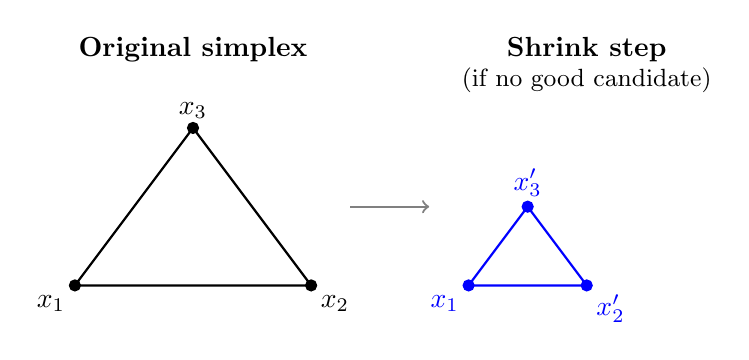
\begin{tikzpicture}[scale=1.0]
    % Original simplex
    \begin{scope}[shift={(0,0)}]
        \node at (1.5, 3) {\textbf{Original simplex}};
        \coordinate (A) at (0,0);
        \coordinate (B) at (3,0);
        \coordinate (C) at (1.5, 2);
        
        \draw[thick] (A) -- (B) -- (C) -- cycle;
        \filldraw (A) circle (2pt) node[below left] {$x_1$};
        \filldraw (B) circle (2pt) node[below right] {$x_2$};
        \filldraw (C) circle (2pt) node[above] {$x_3$};
    \end{scope}
    
    % Arrow between the two simplexes (in global coordinates)
    \draw[->, thick, gray] (3.5, 1) -- (4.5, 1);
    
    % Shrink case (no good candidate)
    \begin{scope}[shift={(5,0)}]
        \node at (1.5, 3) {\textbf{Shrink step}};
        \node at (1.5, 2.6) {\small (if no good candidate)};
        \coordinate (A2) at (0,0);
        \coordinate (B2) at (1.5, 0);
        \coordinate (C2) at (0.75, 1);
        
        \draw[thick, blue] (A2) -- (B2) -- (C2) -- cycle;
        \filldraw[blue] (A2) circle (2pt) node[below left] {$x_1$};
        \filldraw[blue] (B2) circle (2pt) node[below right] {$x_2'$};
        \filldraw[blue] (C2) circle (2pt) node[above] {$x_3'$};
    \end{scope}
\end{tikzpicture}
\caption{Shrink operation towards the best point $x_1$.}
\label{fig:nelder-mead-shrink}
\end{figure}

\begin{figureexplanation}
Figure~\ref{fig:nelder-mead-shrink} illustrates the shrink operation. When none of the candidate points $\bar{x}(-2), \bar{x}(-1), \bar{x}(-\frac{1}{2}), \bar{x}(\frac{1}{2})$ improves the function, the simplex is shrunk towards the best vertex $x_1$.
\end{figureexplanation}

\subsection{Remarks}

\begin{remarque}
The evaluation order $\bar{x}(\frac{1}{2}), \bar{x}(-\frac{1}{2}), \bar{x}(-1), \bar{x}(-2)$ is fairly standard in implementations.
\end{remarque}

\begin{remarque}
Unless the shrinkage step is performed, the quantity
\begin{equation}
    \frac{1}{n+1} \sum_{i=1}^{n+1} f(x_i)
\end{equation}
decreases at each step.
\end{remarque}

\begin{remarque}
For convergence theory, see \cite{kelley1999detection} or \cite{lagarias1995convergence}.
\end{remarque}

\subsection{Algorithm 15: Nelder-Mead Method}

\begin{algorithm}[H]
\caption{One step of the Nelder-Mead Method}
\label{alg:nelder-mead}
Compute the reflection point $\bar{x}(-1)$ and evaluate $f_{-1} = f(\bar{x}(-1))$\;
\If{$f(x_1) \le f_{-1} < f(x_n)$}{
    \Comment*[l]{Reflected point is neither best nor worst in the new simplex}
    Replace $x_{n+1}$ by $\bar{x}(-1)$ and go to the next iteration\;
}
\ElseIf{$f_{-1} < f(x_1)$}{
    \Comment*[l]{Reflected point is better than the current best, try to go further along this direction}
    Compute the expansion point $\bar{x}(-2)$ and evaluate $f_{-2} = f(\bar{x}(-2))$\;
    \If{$f_{-2} < f_{-1}$}{
        Replace $x_{n+1}$ by $\bar{x}(-2)$ and go to the next iteration\;
    }
    \Else{
        Replace $x_{n+1}$ by $\bar{x}(-1)$ and go to the next iteration\;
    }
}
\ElseIf{$f_{-1} \ge f(x_n)$}{
    \Comment*[l]{Reflected point is still worse than $x_n$, contract}
    \If{$f(x_n) \le f_{-1} < f(x_{n+1})$}{
        \Comment*[l]{try to perform ``outside'' contraction}
        Evaluate $f_{-1/2} = f(\bar{x}(-1/2))$\;
        \If{$f_{-1/2} \le f_{-1}$}{
            Replace $x_{n+1}$ by $\bar{x}(-1/2)$ and go to the next iteration\;
        }
    }
    \Else{
        \Comment*[l]{Try to perform ``inside'' contraction}
        Evaluate $f_{1/2} = f(\bar{x}(1/2))$\;
        \If{$f_{1/2} < f(x_{n+1})$}{
            Replace $x_{n+1}$ by $\bar{x}(1/2)$ and go to the next iteration\;
        }
    }
    \Comment*[l]{Neither outside nor inside contraction was acceptable, shrink the simplex toward $x_1$}
    Replace $x_i \leftarrow \frac{1}{2}(x_1 + x_i)$ for $i = 2, 3, \ldots, n+1$\;
}
\end{algorithm}

\subsection{Illustration on the Rosenbrock Function}

\begin{figure}[H]
\centering

\includegraphics[width=0.7\textwidth]{6.png}
\caption{Iterations of the Nelder-Mead simplex method on the level curves of the Rosenbrock function.}
\label{fig:nelder-mead-rosenbrock}
\end{figure}

\begin{figureexplanation}
\textbf{Key points to observe:}
\begin{itemize}
    \item \textbf{Derivative-free method:} Nelder-Mead does not use any information about the gradient, only evaluations of $f$. The trajectory is therefore less direct than Newton or BFGS.
    \item \textbf{Progression in the valley:} We can observe how the simplex deforms and adapts to the geometry of the Rosenbrock valley through successive reflections and contractions.
    \item \textbf{Robustness vs efficiency:} The method converges despite the absence of derivatives, but the number of evaluations of $f$ is much higher than steepest descent (because all other methods also use the gradient).
    \item \textbf{Use case:} This method is particularly useful when the derivatives are unavailable or too expensive to compute (simulations, experimental measurements).
\end{itemize}
\end{figureexplanation}

\bigskip
\begin{checkpoint}
\begin{itemize}
    \item \textbf{Finite differences:} What is the trade-off to find for the choice of the step size $\epsilon$ (Truncation Error vs Noise)?
    \item \textbf{Nelder-Mead:} Name the three main geometric operations on the simplex (Reflection, Expansion, Contraction).
    \item \textbf{Pattern Search:} What condition on the directions ensures convergence?
\end{itemize}
\end{checkpoint}
